\documentclass[12pt,a4paper]{article}
\usepackage{times}
\usepackage[utf8]{inputenc}
\usepackage[czech]{babel}
\usepackage[left=1.5cm, top=1.5cm, text={18cm, 26cm}]{geometry}
\usepackage{graphicx} % figures (\includegraphics...)
\usepackage{float} % figures positioning ([H])
\usepackage[unicode]{hyperref}
\urlstyle{same}
\renewcommand{\figurename}{Obrázek}

\usepackage{amsfonts} % natural numbers -> \mathbb{N}

\usepackage{fancyhdr}
\pagestyle{fancy}
\fancyhf{}
\renewcommand{\headrulewidth}{0pt}

\lfoot{PRL Projekt}
\rfoot{Michal Sova}
\cfoot{\thepage}

%\title{Projekt do předmětu PRL - Odd-Even Merge Sort}
%\author{Michal Sova (xsovam00@stud.fit.vutbr.cz)}

\begin{document}
%\maketitle

\section{Odd-Even Merge Sort}
\label{sec:odd_even_merge_sort}
Základní jednotkou algoritmu Odd-Even Merge Sort je komparátor (Obr. \ref{fig:net1x1}). 
Ten obdrží dva vstupy, a vrací dva výstupy. Jedinou operací komarátoru je porovnat tyto dva vstupy a na výstup dát seřazenou posloupnost těchto dvou vstupů.
Použitím těchto komarátorů lze vytvořit síť, která má na vstupu dvě seřazené posloupnosti $A = \{a_1, a_2, ..., a_n\}$ a $B = \{b_1, b_2, ..., b_n\}$ a na výstupu má seřazenou posloupnost $C = \{c_1, c_2, ..., c_{2n}\}$, kde $n$ je mocninou 2. 
Pro seřazení dvou již seřazených posloupností $A = \{a_1, a_2\}$ a $B = \{b_1, b_2\}$ lze použít síť na Obr. \ref{fig:net2x2}. 
Tímto způsobem lze sestavit kaskádu sítí pro seřazení $2^m$ čísel, kde $m \in \mathbb{N}$ čísel. 
Na Obr. \ref{fig:oems} lze vidět případ Odd-Even Merge Sor pro 8 čísel.
\begin{figure}[H]
\centering
    \begin{minipage}{.45\textwidth}
        \centering
        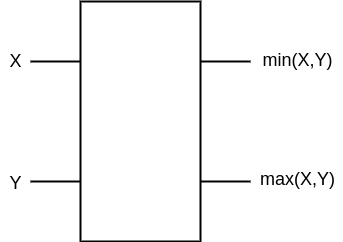
\includegraphics[width=.9\textwidth]{img/comparator.png}
        \caption{Komparátor}
        \label{fig:net1x1}
    \end{minipage}
    \hfill
    \begin{minipage}{.5\textwidth}
        \centering
        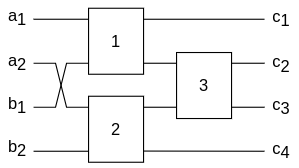
\includegraphics[width=.9\textwidth]{img/net2x2.png}
        \caption{Síť $2\times2$}
        \label{fig:net2x2}
    \end{minipage}
\end{figure}

\subsection*{Časová složitost}
\label{sub:casova_slozitost}
Uvažujme, že komparátor načítá svůj vstup, porovnává ho a generuje výstup v jednu časovou jednotku. 


\subsection*{Počet procesorů}
\label{sub:pocet_procesoru}


\subsection*{Celková cena}
\label{sub:celkova_cena}


\section{Implementace}
\label{sec:implementace}
Propojení jednotlivých procesů, jejich synchronizaci a celkové fungování systému pro osm hodnot na vstupu.



\begin{figure}[H]
    \centering
    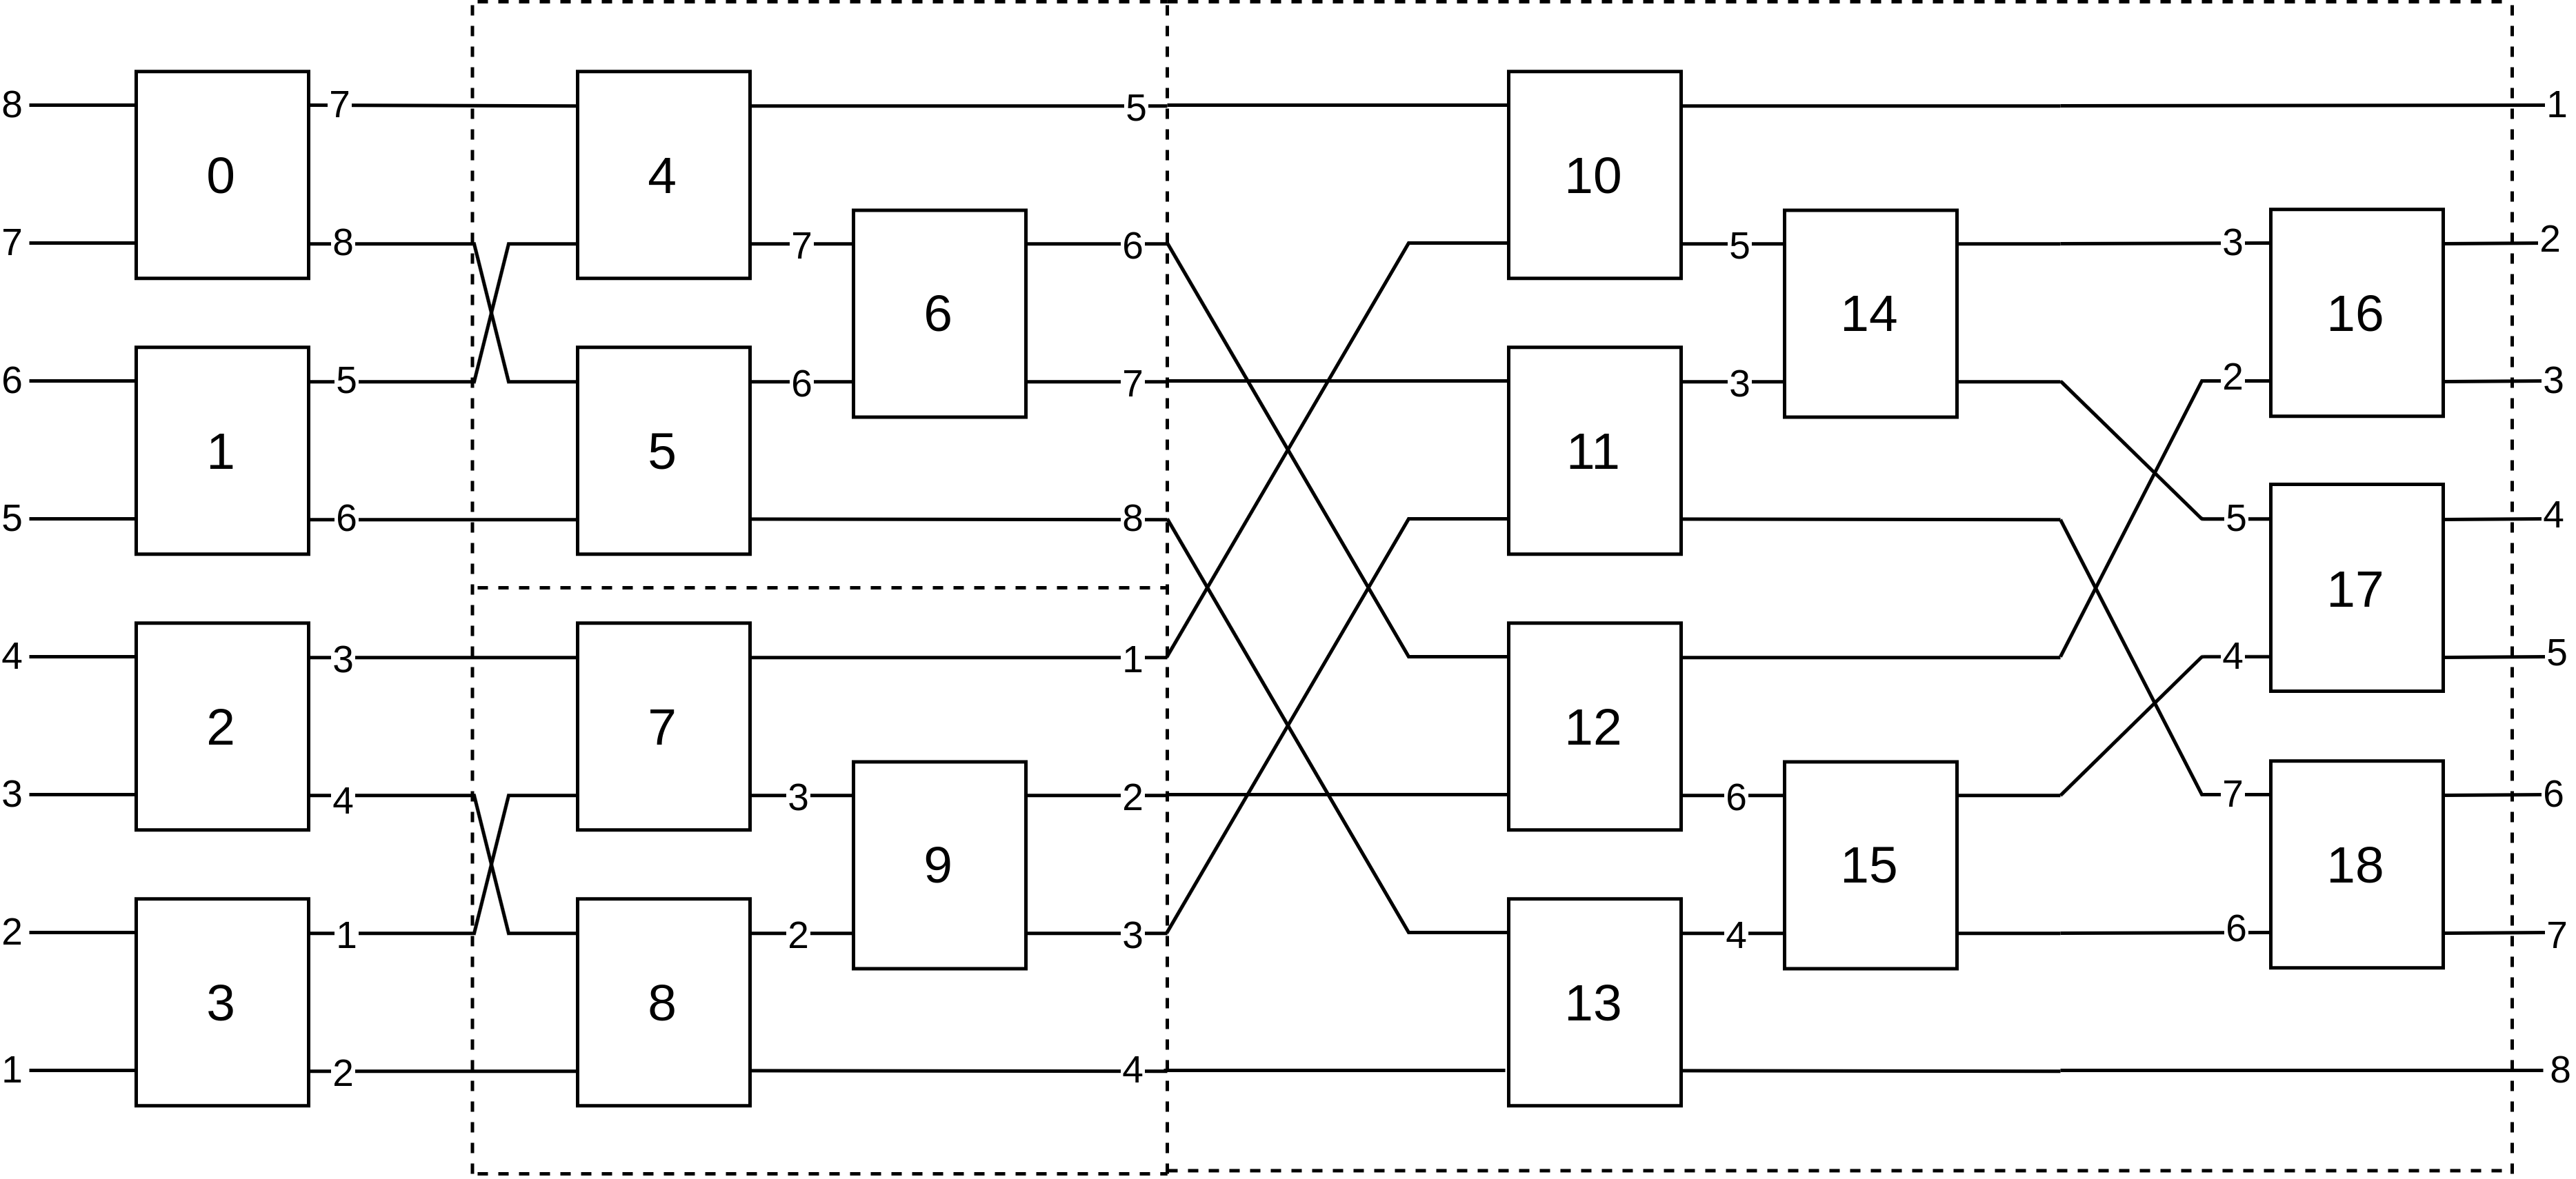
\includegraphics[width=\textwidth]{img/oems.png}
    \caption{Odd-Even Merge Sort pro 8 čísel}
    \label{fig:oems}
\end{figure}

\section{Závěr}
\label{sec:závěr}
Závěr, ve kterém zhodnotíte dosažené výsledky.


\end{document}
